\section{5-(Pentafluorophenyl)dipyrromethan}
\begin{figure}[!htpb]
\centering
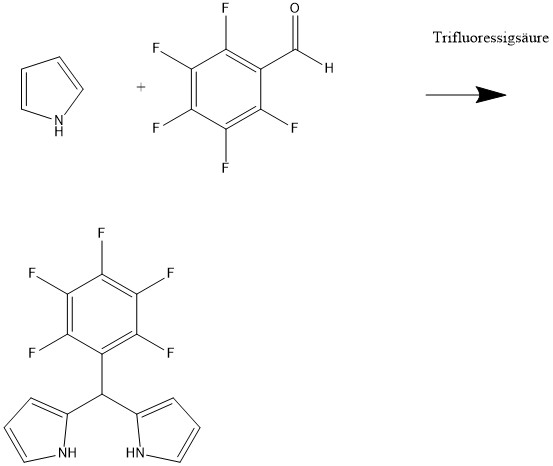
\includegraphics[scale=0.5]{graphics/5-(Pentafluorphenyl)dipyrromethan}
\caption{Synthese von 5-(Pentafluorophenyl)dipyrromethan}
\end{figure}
Das Produkt dient als Vorlage für einen Porphyrinkomplex. Die Reaktion lief wie erwartet, jedoch war die Aufreinigung etwas aufwendiger. Das Pyridin konnte nur mittels Extraktion entfernt werden und nicht mittels Chromatographiesäule. Das Spektrum (siehe \ref{5pfdpmnmr1}) wurde direkt nach der Reaktion ohne Aufreinigung aufgenommen. Die Peaks für die Pyrrolverunreinigungen sind bei 6,82; 6,26 und 5,8. Die restlichen Peaks zeigen den Pyrrolring. Das Lösungsmittelsignal ist bei ca. 7,3. Das Verhältnis von Pyrrol zu Produkt liegt bei 50\%. Nach einmaliger Aufreinigung mittels Kieselgelsäure ist noch immer  viel Pyrrol vorhanden (ca.30\%) Beim Extrahieren mit 40\% Ethanol-Lösung konnte das Pyrrol fast vollständig entfernt werden.
\section{di-(pentafluoro)-di-(Phenyl-Propinyl)porphyrin}
\begin{figure}[!htpb]
\centering
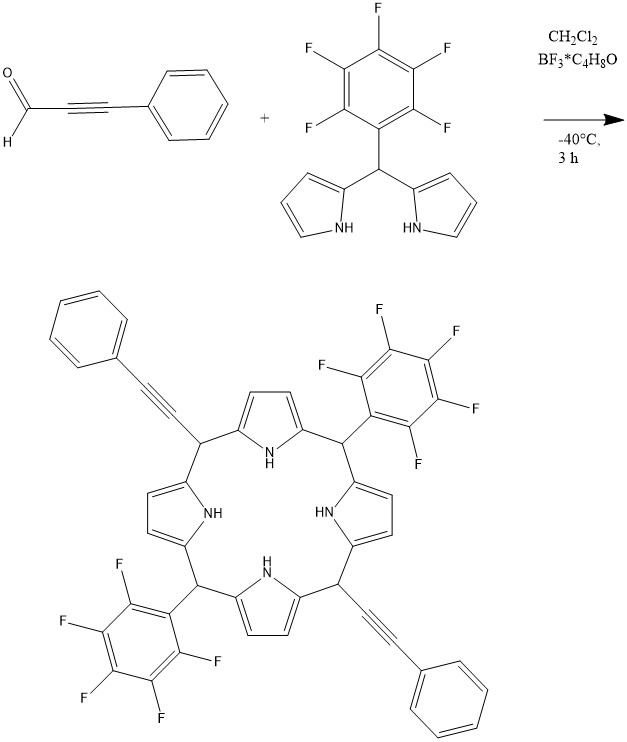
\includegraphics[scale=0.5]{graphics/bis(pentafluorphenyl)-bis(phenylpropinyl)porphyrin}
\caption{Synthese von di-(pentafluoro-die-(Phenylpropinyl)porphyrin}
\end{figure}
Der Komplex wurde laut Paper \cite{16} %%blabla 
mit leicht geänderten Seitenketten hergestellt, da die Synthese recht interessant ausgesehen hatte und der Porphyrinkomplex möglicherweise gute Fluoreszenzeigenschaften gehabt hätte. Im Absorptionsspektrum konnte das Produkt nur gering (leichter Bogen bei 650 nm) bis gar nicht nachgewiesen werden.
Die Lösung blieb nach der Reaktion schwarz und es war kein Porphyrin im Spektrum zu sehen. Vermutlich ist das Produkt während der Reaktion zerfallen oder es konnte nicht stabilisiert werden.

\section{tetra(propinyl)tetra(3,4 diethylpyrrol)}
\begin{figure}[!htpb]
\centering
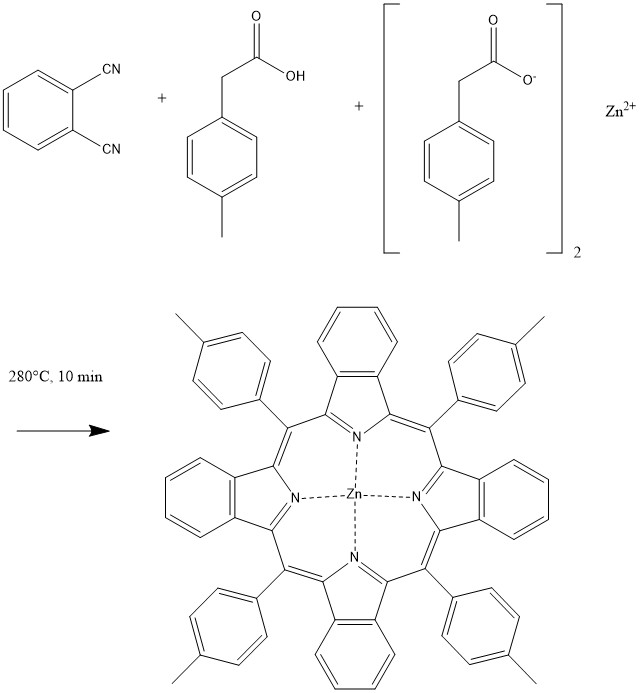
\includegraphics[scale=0.5]{graphics/tetrakis(methylphenyl)tetrakis(phenylpyrrolporphyrin}
\end{figure}
Diese Reaktion wurde genau nach Anleitung \cite{[16]} gemacht, mit den gleichen Edukten und Produkten. Jedoch konnte nur wenig Prophyrin nachgewiesen werden. Das Spektrum hat Bögen. Die Lösung war nach der Reaktion schwarz und hatte keine charakteristische Farbe eines Porphyrins. Das Produkt ist zerfallen oder konnte gar nicht hergestellt werden.
\section{Zinktolylacetat}
\begin{figure}[!htpb]
\centering
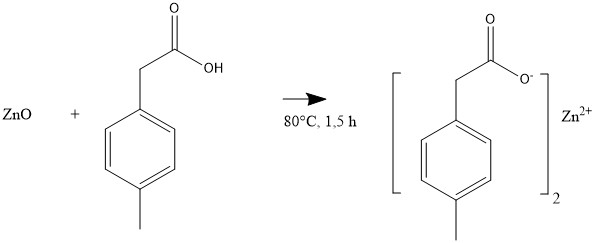
\includegraphics[scale=0.5]{graphics/zinktolylacetat}
\end{figure}
Das zweifach geladene Zinktolylacetat wurde zum Einbau von Zink in den Komplex hergestellt.
Das Produkt und das Edukt wurden anschließend für die Herstellung eines Porphyrinringes verwendet. Da die Reaktion vergleichsweise einfach war und hohe Ausbeuten erwartet werden, wurde auf eine Reaktionskontrolle verzichtet. 
\section{Zn-tetra(tolyl)tetrabenzoporphyrin}
\begin{figure}[!htpb]
\centering
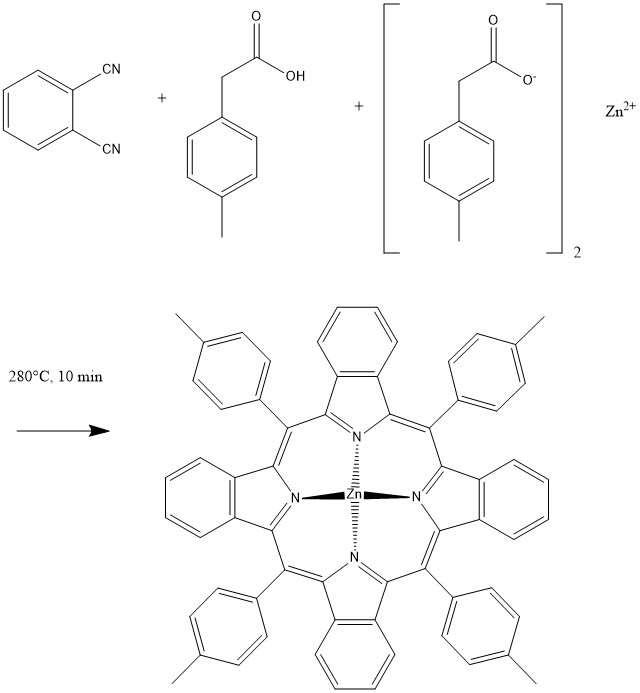
\includegraphics[scale=0.5]{graphics/ZnTtolyltbp}
\end{figure}
Der Zink-Porphyrinkomplex wurde wegen möglicher guter Fluoreszenzeigenschaften hergestellt. Die Methylgruppe am Benzolring soll zusätzlich Löslichkeit bringen, da Porphyrine wegen ihrer Größe grundsätzlich schlechter löslich sind. 
Im NMR-Spektrum erkennt man Peaks bei 8,25 (Multiplett), 7,6(Multiplett); 7,5 (m); 7,25(m); 7,2 (Singlett) und 2,5. Das Spektrum wurde in $C_6D_6$ aufgenommen (Peak bei 7,2). Das Produkt ist ausreichend vorhanden.
\newpage
\section{tetra(tolyltetrabenzoporphyrin}
\begin{figure}[!htpb]
\centering
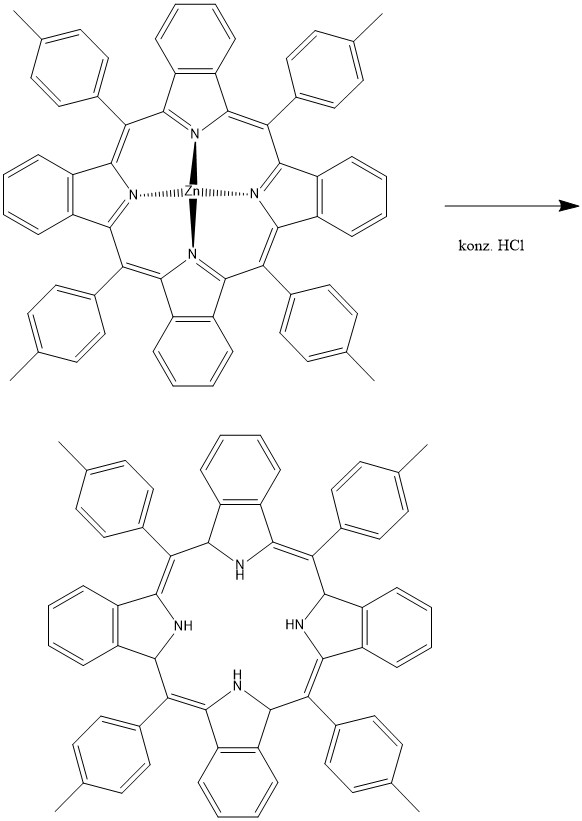
\includegraphics[scale=0.5]{graphics/demetoftetramehtphen}
\end{figure}
Die Demetallierung wurde durchgeführt um Zink aus dem Komplex zu entfernen und später Platin einzuführen. Nach der Reaktion war jedoch kaum Produkt im Spektrum zu erkennen. Die Massenberechnung nach Lambert-Beer'schen Gesetz ($A=\epsilon*c*d$) ergab nur 2,4 mg Produkt. Das kann daran liegen, dass das Produkt beim Filtrieren am Filterpapier hängengeblieben ist, weil es schwer löslich war. Daher ist es als Farbstoff ungeeignet und die Reaktion wurde abgebrochen.
\newpage
\section{ZnmonoOEttriFPhenTBP}
\begin{figure}[!htpb]
\centering
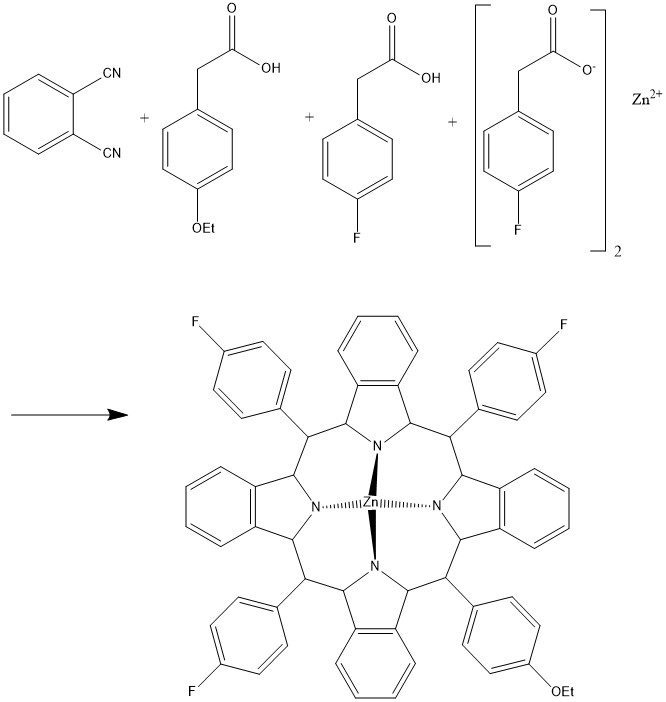
\includegraphics[scale=0.5]{graphics/Zn(ethoxyphenyl)tris(fluorophenyl)tetrakis(phenylpyrrol)porphyrin}
\end{figure}
Ziel dieser Reaktion war es, einen Porphyrinkomplex mit einer Phenyl-O-Ethyl-Gruppen und drei Fluor-Phenyl-Gruppen zu synthetisieren.  Das H-NMR-Spektrum wurde in $CDCl_3$ aufgenommen (Peak bei 7,3). Man erkennt mehrere Singlett-Peaks (8,4;8,2;7,5;4,4; und 1,7) und ein Multiplett bei 7,4. Laut Spektrum haben sich eher Porphyrine mit 2 Phenyl-O-Ethyl-Gruppen und 2 Fluor-Phenylgruppem gebildet, was mit der Abmischung der Edukte zusammenhängen könnte.

\section{mono(O-ethylphenyl)tris(fluorophenyl)tetrabenzoporphyrin}
\begin{figure}[!htpb]
\centering
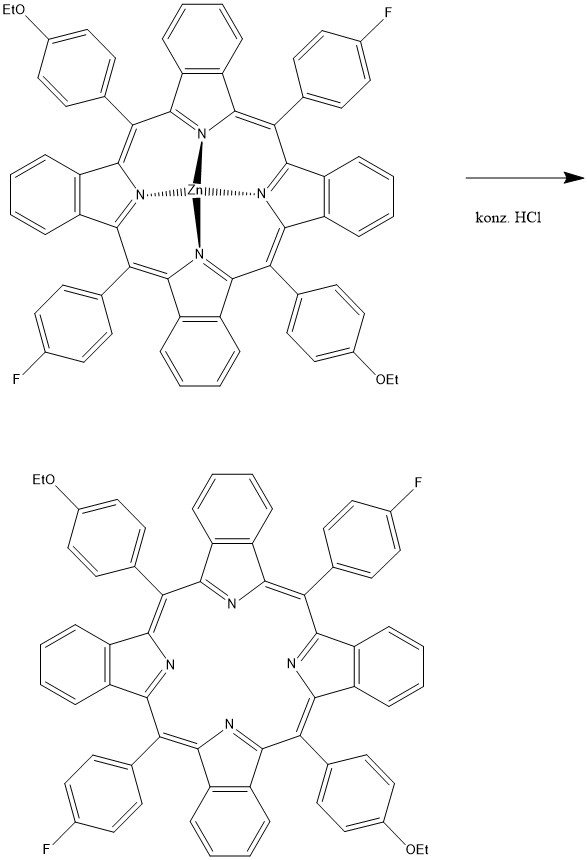
\includegraphics[scale=0.5]{graphics/entmetZnmonoettrifphenTBP}
\end{figure}
Zur Entfernung des Zink als Zentralatom und um dann später eine Platinierung durchzuführen, wurde die Demetallierung mit konzentrierter Salzsäure durchgeführt. Eine Reaktionskontrolle erfolgte nicht.


\section{PtmonoOEttrFPhenTBP}
\begin{figure}[!htpb]
\centering
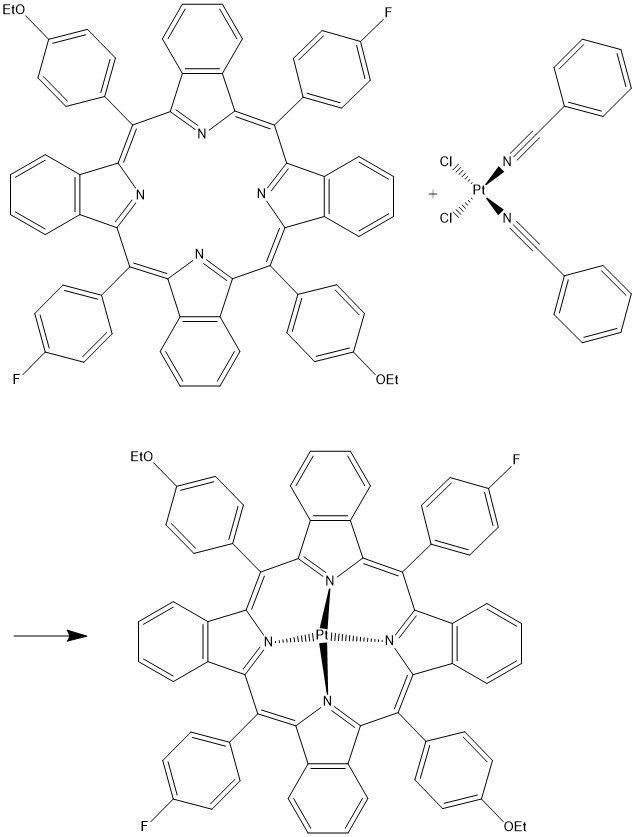
\includegraphics[scale=0.5]{graphics/Platinierung}
\end{figure}
Die Platinierung (Einführung von Platin als Zentralatom in den demetallierten Komplex) wurde durchgeführt, weil Pt-Komplexe stabiler sind und das Absorptionsspektrum nach rechts (naher Infrarotbereich) verschoben wird.
Nach der Platinierung wurde eine Säulenchromatographie zur Aufreinigung gemacht. Jedoch stellte sich laut Spektrum die Trennung der einzelnen Komponenten als schwierig heraus, da bei Aufnahme des Spektrums bei den einzelnen Fraktionen mehrere Peaks erkennbar sind. Mittels Säulenchromatographie könnte kein reines Produkt erhalten werden. Es gibt zwei Hauptpeaks bei 479 nm und bei 645 nm. Dazwischen sind kleinere Peaks zu sehen, die noch auf Nebenprodukte hindeuten. Deswegen wurde an dieser Stelle abgebrochen.

\section{Schollreaktion}
\subsection{Pt(II)tertbutylbenzoporphyrin}
\begin{figure}
\centering
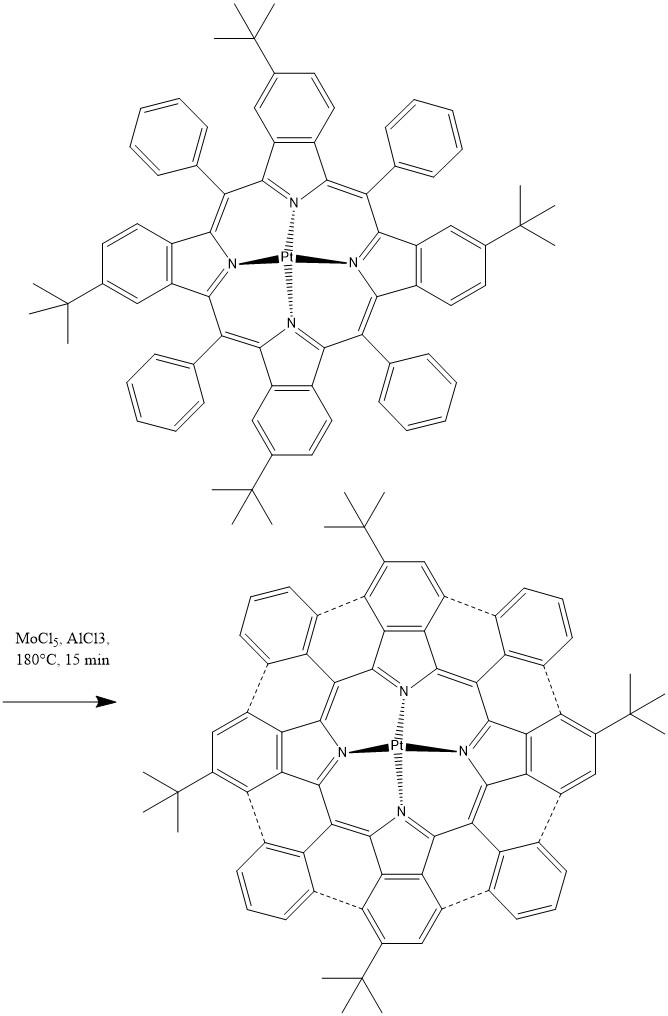
\includegraphics[scale=0.5]{graphics/PttBuTBPreaction}
Die Verbrückung erfolgte um das Spektrum des Komplexes naxh rechts zu verschieben
\end{figure}
\begin{figure}[!htpb]
\centering
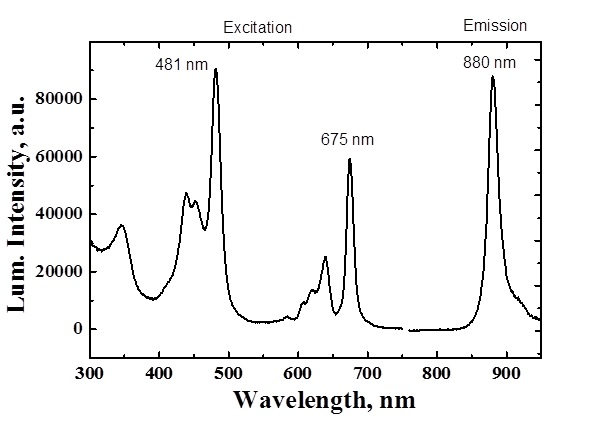
\includegraphics[scale=0.5]{graphics/PttBuTBPafterschollreaction}
\caption{Fluoreszenzspektrum von PttBuTBP nach der Schollreaktion}
\end{figure}
Die Anregung erfolgte bei 481 nm und die Emission bei 880 nm. Die Peaks bei 481 und 675 nm sind sehr spitz und ihnen gehen geringere Spitzen vorraus. Die Emission bei 880 nm weist ebenfalls einen spitzen Peak auf. Damit liegt das Emissionsspektrum im nahen Infrarot-Bereich.


\begin{figure}[!htpb]
\centering
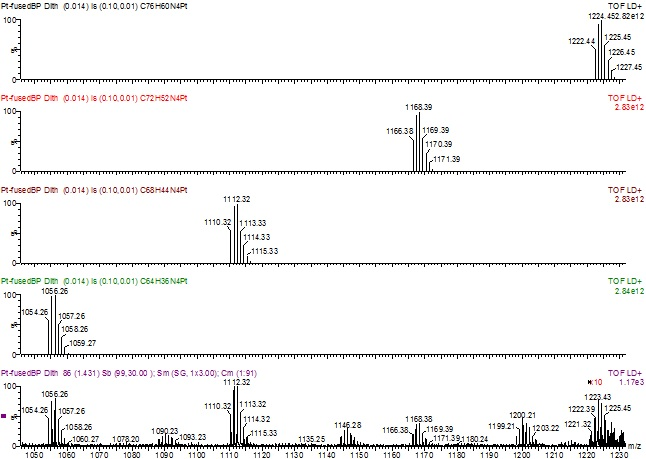
\includegraphics[scale=1]{graphics/PttBuTBPmassspktrum2}
\caption{theoretisches Massenspektrum von PttBuTBP}
\end{figure}

Im Bild sind die theoretischen Isomere der verschieden verbrückten Benzoporphyrinen zu sehen. Mit jeder Schließung eines Ringes geht auch eine Butyl-Gruppe weg.  Die Butyl-Gruppen wurden für die Löslichkeit eingebaut, aber wahrscheinlich werden sie bei hohen Temperaturen abgespalten. Von oben nach unten ist jeweils ein, zwei, drei oder vier Phenylringe komplett miteinander verbrückt sind. Das letzte Spektrum zeigt die experimentell gefundenen Massenspektren. Dabei sieht man, dass ich dreifach und vierfach verbrückte Benzoporphyrine bilden und einfach und zweifach eher nicht bilden. Es sind auch Isotope zwischen den einzelnen Massen zu erkennen.

\begin{figure}[!htpb]
\centering
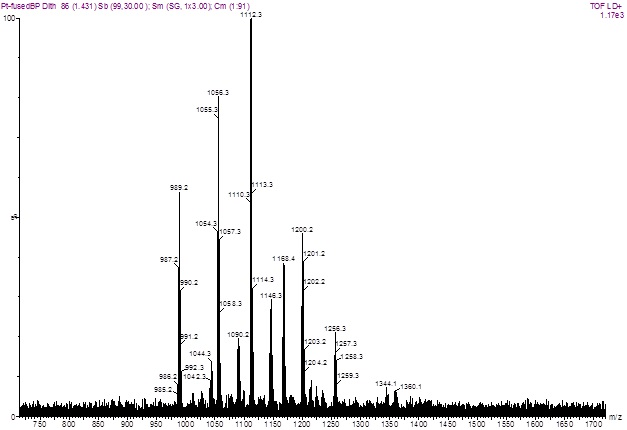
\includegraphics[scale=0.9]{graphics/PttBuTBPmassspktrum1}
\caption{Massenspektrum von PttBuTBP}
\end{figure}
Das unverbrückte Edukt hatte eine Masse von 1280 g/mol. Rechnet man jeweils 56 g/mol (tert-Butylgruppe) weg, so ergeben sich Massen von 1224, 1168, 1112 und 1056 g/mol. Diese scheinen teilweise auch im Spektrum auf. Manchmal hat sich auch ein Cl-Atom eingebaut, was Massen von 1256 und 1200 erklärt, sowie bei 1090 und 1046. Die Masse bei 989 g/mol ist unerklärlich, vermutlich wurde das Metallion entfernt.
Es haben sich mehrere Produkte mit verschieden verbrückten Phenylringen gebildet. Die Trennung dieser Produkte und die genaue Strukturanalyse wird noch eine Herausforderung in Zukunft  sein. Wenn man mit dem Porphyrin Kristallstrukturen bilden könnte, so kann die Struktur mit Röntgenstrukturanalyse herausgefunden werden. Eine Trennung und Isolierung ist vielleicht mit Säulenchromatographie möglich.
\newpage
\subsection{PttBumonoAzaTBP}
\begin{figure}[!htpb]
\centering
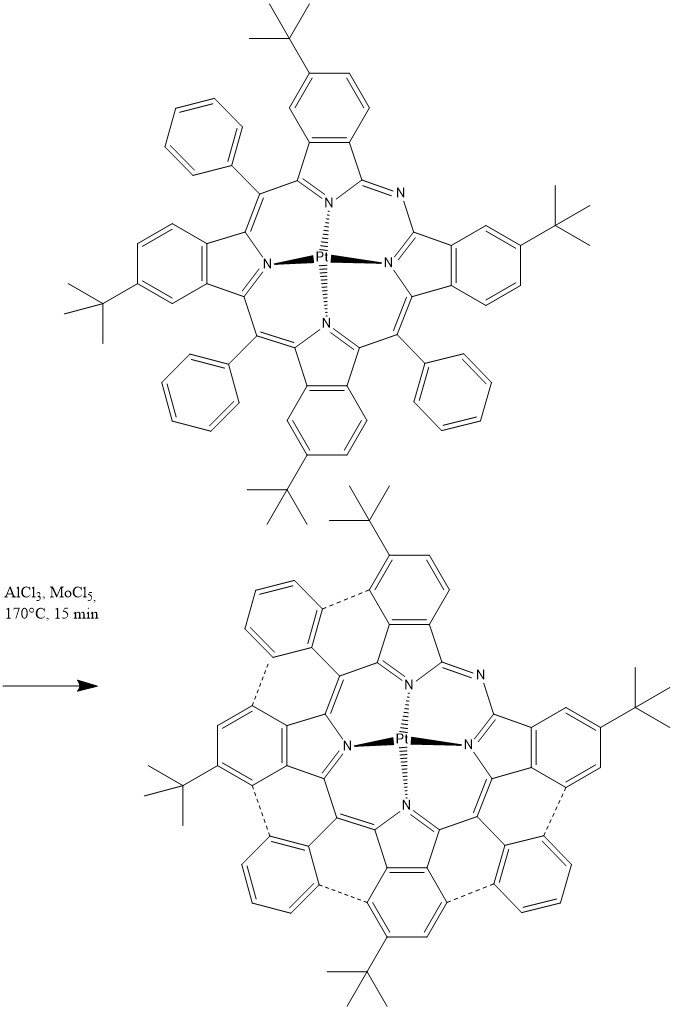
\includegraphics[scale=0.5]{graphics/PttBumonoAzaTBPreaction}
\end{figure}
Die Verbrückung erfolgte ähnlich wie beim oberen Beispiel. Das Edukt besitzt drei Phenylringe und statt eines vierten Phenylringes hat es eine Stickstoffbrücke. 

Im Fluoreszenzspektrum (\ref{Anregmononaza}) erkennt man zwischen 390 und 480 nm  einen breiten Bereich mit zwei leichten Peaks. Dieser ist undefinerter als der im vorhergehenden Beispiel. Zwischen 600 nm und 670 nm erkennt man drei Peaks, von denen der mit 660 nm der höchste und sehr spitz ist.


Die Emission (\ref{emissmonoaza}) liegt mit 925 nm im nahen Infrarot-Bereich. Es gibt nur einen Peak, der sehr spitz ist. Damit ist dieses Produkt als Indikator geeignet.